\documentclass[12pt,a4paper,openany]{book}

\usepackage{lmodern}
\usepackage{xcolor}
\usepackage{xcolor}
\definecolor{vert1}{rgb}{0.0,0.3.9,0.0}
\definecolor{bleu}{rgb}{0,0,0.5}
\definecolor{bleu3}{rgb}{1,0.2,0.2}
\definecolor{grisgris}{gray}{0.4}
\definecolor{grisclair}{HTML}{E7E7E7}
\definecolor{grisfonce}{HTML}{A5A5A5}
\definecolor{rougeUPS}{rgb}{0.6, 0.3, 0.3}

\fboxsep =0pt \parindent =0pt\parskip =12pt



\usepackage[utf8]{inputenc}
\usepackage[T1]{fontenc}
\usepackage[francais]{babel}
\usepackage[top=1.7cm, bottom=1.7cm, left=1.7cm, right=1.7cm]{geometry}
\usepackage{verbatim}
\usepackage[urlbordercolor={1 1 1}, linkbordercolor={1 1 1}, linkcolor=vert1, urlcolor=bleu, colorlinks=true]{hyperref}
\usepackage{tikz} %Vectoriel
\usepackage{listings}
\usepackage{fancyhdr}
\usepackage{multido}
\usepackage{amssymb}
\usepackage{float}

\newcommand{\titre}{Algorithmie en langage C}

\newcommand{\pole}{}
\newcommand{\sigle}{algo}

\newcommand{\semestre}{3}

\definecolor{gris1}{gray}{0.40}
\definecolor{gris2}{gray}{0.55}
\definecolor{gris3}{gray}{0.65}
\definecolor{gris4}{gray}{0.50}
\definecolor{vert}{rgb}{0,0.4,0}
\definecolor{violet}{rgb}{0.65, 0.2, 0.65}
\definecolor{bleu1}{rgb}{0,0,0.8}
\definecolor{bleu2}{rgb}{0,0.2,0.6}
\definecolor{bleu3}{rgb}{0,0.2,0.2}
\definecolor{rouge}{HTML}{F93928}


\lstdefinelanguage{algo}{%
   morekeywords={%
    %%% couleur 1
		importer, programme, glossaire, fonction, procedure, constante, type, 
	%%% IMPORT & Co.
		si, sinon, alors, fin, tantque, debut, faire, lorsque, fin lorsque, 
		declenche, declencher, enregistrement, tableau, retourne, retourner, =, pour, a,
		/=, <, >, traite,exception, 
	%%% types 
		Entier, Reel, Booleen, Caractere, Réél, Booléen, Caractère,
	%%% types 
		entree, maj, sortie,entrée,
	%%% types 
		et, ou, non,
	},
  sensitive=true,
  morecomment=[l]{--},
  morestring=[b]',
}

\lstset{language=algo,
    %%% BOUCLE, TEST & Co.
      emph={importer, programme, glossaire, fonction, procedure, constante, type},
      emphstyle=\color{bleu2},
    %%% IMPORT & Co.  
	emph={[2]
		si, sinon, alors, fin , tantque, debut, faire, lorsque, fin lorsque, 
		declencher, retourner, et, ou, non,enregistrement, retourner, retourne, 
		tableau, /=, <, =, >, traite,exception, pour, a
	},
      emphstyle=[2]\color{bleu1},
    %%% FONCTIONS NUMERIQUES
      emph={[3]Entier, Reel, Booleen, Caractere, Booléen, Réél, Caractère},
      emphstyle=[3]\color{gris1},
    %%% FONCTIONS NUMERIQUES
      emph={[4]entree, maj, sortie, entrée},	
      emphstyle=[4]\color{gris1},
}
\lstdefinelanguage{wl}{%
   morekeywords={%
    %%% couleur 1
		importer, programme, glossaire, fonction, procedure, constante, type, 
	%%% IMPORT & Co.
		si, sinon, alors, fin, TANTQUE, tantque, FIN, PROCEDURE, debut, faire, lorsque, 
		fin lorsque, declenche, declencher, enregistrement, tableau, retourne, retourner, =, 
		/=, <, >, traite,exception, 
	%%% types 
		Entier, Reel, Booleen, Caractere, Réél, Booléen, Caractère,
	%%% types 
		entree, maj, sortie,entrée,
	%%% types 
		et, ou, non,
	},
  sensitive=true,
  morecomment=[l]{//},
  morestring=[b]',
}

\lstset{language=wl,
    %%% BOUCLE, TEST & Co.
      emph={importer, programme, glossaire, fonction, procedure, constante, type},
      emphstyle=\color{bleu2},
    %%% IMPORT & Co.  
	emph={[2]
		si, sinon, alors, fin , tantque, debut, faire, lorsque, fin lorsque, 
		declencher, retourner, et, ou, non,enregistrement, retourner, retourne, 
		tableau, /=, <, =, >, traite,exception
	},
      emphstyle=[2]\color{bleu1},
    %%% FONCTIONS NUMERIQUES
      emph={[3]Entier, Reel, Booleen, Caractere, Booléen, Réél, Caractère},
      emphstyle=[3]\color{gris1},
    %%% FONCTIONS NUMERIQUES
      emph={[4]entree, maj, sortie, entrée},	
      emphstyle=[4]\color{gris1},
}
\lstdefinelanguage{css}{%
   morekeywords={%
    %%% couleur 1
		background, image, repeat, position, index, color, border, font, 
		size, url, family, style, variant, weight, letter, spacing, line, 
		height, text, decoration, align, indent, transform, shadow, 
		background, image, repeat, position, index, color, border, font, 
		size, url, family, style, variant, weight, letter, spacing, line, 
		height, text, decoration, align, indent, transform, shadow, 
		vertical, align, white, space, word, spacing,attachment, width, 
		max, min, margin, padding, clip, direction, display, overflow,
		visibility, clear, float, top, right, bottom, left, list, type, 
		collapse, side, empty, cells, table, layout, cursor, marks, page, break,
		before, after, inside, orphans, windows, azimuth, after, before, cue, 
		elevation, pause, play, during, pitch, range, richness, spek, header, 
		numeral, punctuation, rate, stress, voice, volume,
	%%% types 
		left, right, bottom, top, none, center, solid, black, blue, red, green,
	},
  sensitive=true,
  sensitive=true,
  morecomment=[s]{/*}{*/},
  morestring=[b]',
}
\lstset{language=css,
    %%% BOUCLE, TEST & Co.
      emph={
		background, image, repeat, position, index, color, border, font, 
		size, url, family, style, variant, weight, letter, spacing, line, 
		height, text, decoration, align, indent, transform, shadow, 
		background, image, repeat, position, index, color, border, font, 
		size, url, family, style, variant, weight, letter, spacing, line, 
		height, text, decoration, align, indent, transform, shadow, 
		vertical, align, white, space, word, spacing,attachment, width, 
		max, min, margin, padding, clip, direction, display, overflow,
		visibility, clear, float, top, right, bottom, left, list, type, 
		collapse, side, empty, cells, table, layout, cursor, marks, page, break,
		before, after, inside, orphans, windows, azimuth, after, before, cue, 
		elevation, pause, play, during, pitch, range, richness, spek, header, 
		numeral, punctuation, rate, stress, voice, volume,
	  },
      emphstyle=\color{bleu2},
    %%% FONCTIONS NUMERIQUES
      emph={[3]
		left, right, bottom, top,none, solid, black, blue, green,
		  },
      emphstyle=[3]\color{bleu3},
    %%% FONCTIONS NUMERIQUES
}

\lstset{language=SQL,
    %%% BOUCLE, TEST & Co.
      emph={INSERT, UPDATE, DELETE, WHERE, SET, GROUP, BY, ORDER, REFERENCES},
      emphstyle=\color{bleu2},
    %%% IMPORT & Co.  
	emph={[2]
		if, end, begin, then, for, each, else, after, of, on, to
	},
      emphstyle=[2]\color{bleu1},
    %%% FONCTIONS NUMERIQUES
      emph={[3]Entier, Reel, Booleen, Caractere, Booléen, Réél, Caractère},
      emphstyle=[3]\color{gris1},
    %%% FONCTIONS NUMERIQUES
      emph={[4]entree, maj, sortie, entrée},	
      emphstyle=[4]\color{gris1},
}
\lstdefinelanguage{ARM}{%
   morekeywords={%
   ADD, SUB, MOV, MUL, RSB,CMP, BLS, BLE, B,BHI,LDR,
   BGE, RSBLT, BGT, BEQ, BNE,BLT,BHS,STR,STRB
	},
  sensitive=true,
  morecomment=[l]{@},
  morestring=[b]',
}

\lstset{ % general style for listings 
   numbers=left 
   , literate={é}{{\'e}}1 {è}{{\`e}}1 {à}{{\`a}}1 {ê}{{\^e}}1 {É}{{\'E}}1 {ô}{{\^o}}1 {€}{{\euro}}1{°}{{$^{\circ}$}}1 {ç}{ {c}}1 {ù}{u}1
	, extendedchars=\true
   , tabsize=2 
   , frame=l
   , framerule=1.1pt
   , linewidth=520px
   , breaklines=true 
   , basicstyle=\footnotesize\ttfamily 
   , numberstyle=\tiny\ttfamily 
   , framexleftmargin=0mm 
   , xleftmargin=0mm 
   , captionpos=b 
	, keywordstyle=\color{bleu2}
	, commentstyle=\color{vert}
	, stringstyle=\color{rouge}
	, showstringspaces=false
	, extendedchars=true
	, mathescape=true
} 
%	\lstlistoflistings
%	\addcontentsline{toc}{part}{List of code examples}
 %prise en charge du langage C 
\date{\today}

\makeindex
\lfoot{Université Toulouse III -- Paul Sabatier}
\rfoot{\sigle\semestre}
%\rfoot{}
\cfoot{}
\makeglossary
\makeatletter
\def\clap#1{\hbox to 0pt{\hss #1\hss}}%
\def\ligne#1{%
\hbox to \hsize{%
\vbox{\centering #1}}}%
\def\haut#1#2#3{%
\hbox to \hsize{%
\rlap{\vtop{\raggedright #1}}%
\hss
\clap{\vtop{\centering #2}}%
\hss
\llap{\vtop{\raggedleft #3}}}}%
\def\bas#1#2#3{%
\hbox to \hsize{%
\rlap{\vbox{\raggedright #1}}%
\hss \clap{\vbox{\centering #2}}%
\hss
\llap{\vbox{\raggedleft #3}}}}%
\def\maketitle{%
\thispagestyle{empty}\vbox to \vsize{%
\haut{}{\@blurb}{}

\vfill
\vspace{1cm}
\begin{flushleft}
\usefont{OT1}{ptm}{m}{n}
\huge \@title
\end{flushleft}
\par
\hrule height 4pt
\par
\begin{flushright}
\usefont{OT1}{phv}{m}{n}
\Large \@author
\par
\end{flushright}
\vspace{1cm}
\vfill
\vfill
\bas{}{\@location, le \@date}{}
}%
\cleardoublepage
}
\def\date#1{\def\@date{#1}}
\def\author#1{\def\@author{#1}}
\def\title#1{\def\@title{#1}}
\def\location#1{\def\@location{#1}}
\def\blurb#1{\def\@blurb{#1}}
\date{\today}
\author{}
\title{}
\location{Amiens}\blurb{}
\makeatother
\title{\titre}
\author{Semestre \semestre}

\location{Toulouse}
\blurb{%
Université Toulouse III -- Paul sabatier\\
L2 Informatique\\
}%



%\title{Cours \\ \titre}
%\date{\today\\ Semestre \semestre}

%\lhead{Cours: \titre}
%\chead{}
%\rhead{\thepage}

%\lfoot{Université Paul Sabatier Toulouse III}
%\cfoot{\thepage}
%\rfoot{\sigle\semestre}

\pagestyle{fancy}
\renewcommand{\chaptermark}[1]{\markboth{\bsc{\chaptername~\thechapter{} :} #1}{}}
\renewcommand{\sectionmark}[1]{\markright{\thesection{ #1}}}
\renewcommand{\headrulewidth}{0.3pt}
\renewcommand{\footrulewidth}{0.3pt}

\fancyhf{}
\fancyhead[LE]{\leftmark}
\fancyhead[RO]{\rightmark}
\fancyfoot[LE,RO]{--~\thepage~--}
\fancyfoot[LO]{\titre{}~~---~~\sigle{}\semestre{}}
\fancyfoot[RE]{Antoine de \bsc{Roquemaurel}}

%% Cas des premières pages de chapitre
\fancypagestyle{plain}{%
	\fancyhf{}%
	\fancyfoot[L]{\titre{}~~---~~\sigle{}\semestre{}}
	\fancyfoot[R]{--~\thepage~--}
	\renewcommand{\headrulewidth}{0pt}
	\renewcommand{\footrulewidth}{0.3pt}
}
\makeatletter
\renewcommand*{\lstlistlistingname}{Liste des codes sources}
\renewcommand\listoffigures{%
    \chapter{\listfigurename}%
      \@mkboth{\MakeUppercase\listfigurename}%
              {\MakeUppercase\listfigurename}%
       \@starttoc{lof}%
    }
    \renewcommand\listoftables{%
    \chapter{\listtablename}%
    \@mkboth{\MakeUppercase{\listtablename}}%
            {\MakeUppercase{\listtablename}}%
    \@starttoc{lot}
    }

    \renewcommand\lstlistoflistings{%
    \begingroup
    \chapter{\lstlistlistingname}%
    \parskip\z@\parindent\z@\parfillskip \z@ \@plus 1fil%
    \@starttoc{lol}%
    \endgroup
    }
	\makeatother

\newcommand{\remarque}[1]{
	\begin{center}
	\medskip
	\colorbox{remarque}{
		\begin{minipage}{0.85\textwidth}\medskip
\includegraphics[height=10px]{images/remarque.png} #1 \medskip\end{minipage}
	}
	\medskip
	\end{center}
}

\newcounter{exemples}

\newenvironment{exemple}[1]{
   \vspace{-2mm}

\refstepcounter{exemples}
   \begin{center}
	\medskip
      \begin{minipage}{0.9\linewidth}
}{%
~
      \end{minipage}
   \end{center}~
   \vspace{-2mm}
}%

\newcommand{\captionExemple}[1]{
	\begin{center}{\bsc{Exemple} \thechapter.\arabic{exemples}~--~}#1\end{center}
}

\DeclareTextFontCommand{\policeGlossaire}{\fontfamily{lmss}\selectfont}
\DeclareTextFontCommand{\policePackage}{\fontfamily{phv}\selectfont}
\DeclareTextFontCommand{\policeTitre}{\fontfamily{ptm}\selectfont}
\newcommand{\policeCode}[1]{\texttt{#1}}

\newcommand{\sectionfont}{%
	\fontencoding{\encodingdefault}%
	\fontfamily{pag}%
	\fontseries{bc}%
	\fontshape{n}%
	\selectfont
}

% numéro du chapitre
\DeclareFixedFont{\chapnumfont}{T1}{phv}{b}{n}{80pt}
% pour le mot « Chapitre »
\DeclareFixedFont{\chapchapfont}{T1}{phv}{b}{n}{16pt}
% pour le titre
\DeclareFixedFont{\chaptitfont}{T1}{phv}{b}{n}{24.88pt}


\makeatletter
\def\thickhrulefill{\leavevmode \leaders \hrule height 1ex \hfill \kern \z@}
%% \chapter
\def\@makechapterhead#1{%
  \reset@font
  \parindent \z@
  \vspace*{10\p@}%
  \hbox{%
    \vbox{%
      \advance\hsize by -2cm
      \hrule height 0.4pt depth 0pt width \hsize
      \par
      \vskip 6pt%
      \hspace{20pt}%
      \parbox{420pt}{%
        \LARGE \bfseries #1
		}%
      \par
      \vskip 6pt%
      \hspace{20pt}%
      \hrule height 0.4pt depth 0pt width \hsize
	  \vspace{-30pt}
      }%
    \vbox{%
      \hsize=1.5cm%
      \begin{tabular}{c}
        \scshape \large \strut \@chapapp{} \\
        \colorbox{black}{\vbox{\hbox{\vbox to 1mm{}}\hbox{
			\color{white} \LARGE \bfseries \hspace{1mm}\thechapter\hspace{1mm}
		}\hbox{\vbox to 2cm{}}}}%
      \end{tabular}%
      }%
    }%
  \vskip 20\p@
}
%% \chapter*
\def\@makeschapterhead#1{%
  \reset@font
  \parindent \z@
  \vspace*{10\p@}%
  \hbox{%
    \vbox{%
      \advance\hsize by -0cm
      \hrule height 0.4pt depth 0pt width \hsize
      \par
      \vskip 6pt%
      \hspace{20pt}%
      \parbox{420pt}{%
        \LARGE \bfseries #1
		}%
      \par
      \vskip 6pt%
      \hspace{20pt}%
      \hrule height 0.4pt depth 0pt width \hsize
      }%
    }%
  \vskip 20\p@

}

\newlength{\sectiontitleindent}
\newlength{\subsectiontitleindent}
\newlength{\subsubsectiontitleindent}
\setlength{\sectiontitleindent}{-1cm}
\setlength{\subsectiontitleindent}{-.5cm}
\setlength{\subsubsectiontitleindent}{-.25cm}

\renewcommand{\section}{%
	\@startsection%
	{section}%
	{1}%
	{\sectiontitleindent}%
	{-3.5ex plus -1ex minus -.2ex}%
	{2.3ex plus.2ex}%
	{\sectionfont\Large}
}
\renewcommand{\subsection}{%
	\@startsection%
	{subsection}%
	{2}%
	{\subsectiontitleindent}%
	{-3.5ex plus -1ex minus -.2ex}%
	{2.3ex plus.2ex}%
	{\sectionfont\large}
}

\renewcommand{\subsubsection}{%
	\@startsection%
	{subsubsection}%
	{3}%
	{\subsubsectiontitleindent}%
	{-3.5ex plus -1ex minus -.2ex}%
	{2.3ex plus.2ex}%
	{\sectionfont\normalsize}
}

\makeatother



\makeatother

\begin{document}
	\setcounter{tocdepth}{1}
	\setcounter{secnumdepth}{3}
	\maketitle
	\tableofcontents
	\chapter{Paradigmes de programmation}
		Un paradigme est une manière de programmer, il en existe plusieurs: 
		\begin{itemize}
			\item La programmation fonctionnelles (cf. \ref{fonctionnelles})
			\item La programmation déclarative (cf. \ref{declarative})
			\item La programmation impérative (cf. \ref{imperative}
		\end{itemize}
		\section{Programmation fonctionnelles} \label{fonctionnelles}
		\begin{description}
		\item[Type de langage] \footnote{Traduction du langage source vers le langage cible(compilation) + une édition de liens, qui est une instanciation sur la machine d'exécution (Recherche d'adresse, mémoire, résolution de fonctions) Elle peut être statique ou dynamique. Ex: C, Adda} ou interprétés\footnote{
		Le langage source est traduit en langage cible à la volée par un interpréteur. Il est ainsi possible de modifier le programme pendant le fonctionnement du programme.}. Ce paradigme
		\item[Entité de base] Appel de fonction
		\item[Structure de contrôle] Approche récursive. 


		Elle est utilisée pour des systèmes critiques\footnote{Besoin d'une sureté de fonctionnement}. Elle à une approche très mathématiques, ce qui 
		permet d'avoir des outils de preuves générique.

		Elle possède une abstraction de l'environnement d'exécution, approche détachée de la machine, pas de notion de mémoire.

		\exemple{Le Caml est un langage de programmation fonctionnelle}
	\end{description}
	\section{Programmation déclarative} \label{declarative}
		\begin{description}
			\item[Type de langage] Interprété
			\item[Entité de base] Règles de déduction logique.
			\item[Structure de contrôle  ]
			Possède une abstraction de la machine cible.
			\exemple{Le prolog est un langage de programmation déclarative}
		\end{description}
		\newpage
		\section{Programmation Impérative}\label{imperative}
			La programmation est directement liée à la machine d'exécution.
			\begin{description}	
				\item[Type de langage] Compilé ou Interprété
				\item[Entité de base] Affectation d'une valeur à une variable, qui est une place en mémoire.
				\item[Structure de contrôle] Séquence, sélection, répétition.
			\exemple{C, Python, Ada \ldots}
			\end{description}

	\chapter{Programmation impérative en C}
	Énormément de langage sont fondés sur la syntaxe du langage C.

	Il a été développé dans les années 1960 par Dennis Ritchie. 

	On trouvera toujours une partie description de l'organisation des données en mémoire\footnote{C'est un grand tableau découpé en cases mémoire.},
	nous aurons donc une déclaration de variables et un type de données.
	\begin{lstlisting}[caption=Syntaxe de déclaration de variable]
type nomVariable;		
	\end{lstlisting}
	\section{Description de l'organisation des données en mémoire}\label{types}
	Le C possède différents type de données: 
	\begin{description}
		\item[int] Entiers signés
		\item[unsigned int] Entiers non signés 
		\item[float] Nombre réel sur 32bits. 
		\item[double] Nombre réel sur 64bits.
		\item[char] Entier signé sur 8bits.
		\item[pointeur] type* ptr; La case mémoire contient une adresse.
	\end{description}
	\section{Code syntaxe}
	\subsection{Blocs}
\begin{lstlisting}[language=C, caption=Syntaxe d'un bloc]
bloc { // début du bloc
} //fin du bloc
\end{lstlisting}
	Toute variable est visible dans son bloc de déclaration et ses blocs imbriqués.

	Un bloc transforme une séquence en action.

	\subsection{Séquence}
\begin{lstlisting}[language=C, caption=Syntaxe des actions]
action 1;
action 2;
action 3;
\end{lstlisting}
	\subsection{Séléction}
\begin{lstlisting}[language=C, caption=Syntaxe d'une structure de contrôle]
if(conditon) {
	action 1;
} else {
	action 2;
}
\end{lstlisting}
Condition est une expression booléenne\footnote{Expression renvoyant vrai($\neq 0$) ou faux($=0$)}, si celle-ci est vrai, action 1 est executé, sinon action 2 est executé. 

\subsection{Répétition}
\begin{lstlisting}[language=C, caption=Syntaxe de répétition]
while(condition) {
	action;
}
\end{lstlisting}
Condition est une expression booléenne, tant que la condition est vrai, les actions se répètent.

\subsection{Affectation}
\begin{lstlisting}[language=C, caption=Syntaxe d'une affectation ]
variable = expression;
\end{lstlisting}
variable reçoit expression, si celle-ci n'est pas du même type que variable, un cast\footnote{ou conversion de type, consiste à convertir un type vers un autre. (int vers double par exemple)} peut-être effectué.
\subsection{Opérateurs de base sur les types}
\begin{description}
	\item[\texttt{=}] Affectation
	\item[\texttt{+}, \texttt{-}, \texttt{/}, \texttt{*}] Opérateurs arithmétiques.
	\item[\texttt{\&\&}, \texttt{||}, \texttt{!}] Opérateurs logiques 
	\item[\texttt{==}, \texttt{!=}, \texttt{<}, \texttt{>}, \texttt{<=}, \texttt{>=}] Opérateurs booléens
	\item[\texttt{+$\,$+i}, \texttt{i+$\,$+}, \texttt{-$\,$-i}, \texttt{i-$\,$-}] Opérateur unaires d'incrémentation.
\end{description}
\subsection{Opérateurs d'entrées / sorties}
\paragraph{Ecriture}~\\
\begin{lstlisting}[language=C, caption=Syntaxe de l'appel de printf]
printf('format', var1, var2);
\end{lstlisting}
La chaine format peut contenir une chaine de caractères, avec des caractères spéciaux : 
\begin{description}
	\item[\texttt{'\%d'}] Entier sous forme décimale
	\item[\texttt{'\%ox'}] Entier sous forme hexadécimale
	\item[\texttt{'\%f'}] Flottant 
	\item[\texttt{'\%c'}] Caractère 
	\item[\texttt{'\%s'}] Chaine de caractères 
	\item[\texttt{'\\n'}] Vide le buffer et fait un retour chariot 
	\item[\texttt{'\\t'}] Tabulation 
	\item[\texttt{'\\r'}] Revient en début de ligne.
	\item['\ldots'] RTFM	
\end{description}
Les différents formats doivent être dans l'ordre des variables passés en paramètres.
\paragraph{Lecture}~\newline
\begin{lstlisting}[language=C, caption=Syntaxe de l'appel de scanf]
scanf('format', &var1); // & représente l'adresse de la variable dans laquelle écrire.
\end{lstlisting}
\attention{L'utilisation de cette fonction est risquée. En effet, un utilisateur malveillant peut écrire à des cases mémoires où il n'est pas autorisé.}

\subsection{Tableaux}
Un tableau est une collection d'éléments de même type.
\begin{lstlisting}[language=C, caption=Syntaxe de déclaration d'un tableau]
// avec tableau le nom de la variable et N la taille du tableau. 
type tableau[N], i; 
i = tableau[P]; //i recoit la valeur de la case P du tableau
\end{lstlisting}
\attention{Un tableau commence toujours à 0 et finit à N-1, ainsi, il faut faire très attention au dépassement de la taille d'un tableau.}
\subsection{Les sous-programmes}
Un sous-programme est un sous-ensemble du programme dans sa hiérarchie fonctionnelle. En C, il correspond toujours à une fonction ou une procédure.
\begin{lstlisting}[language=C, caption=Syntaxe d'un sous programme]
typeRetour nomFonction (typeArg1 nomArg1, typeArg2 nomArg2) {
	/*
     *	code
	 */
	 [return (valeur)];
}
\end{lstlisting}
\texttt{typeRetour} peut posséder comme valeur les même types qu'une variable, voir \ref{types} page \pageref{types}. Celui-ci peut également être \texttt{void}, 
cela signifie que que la fonction ne renvoie rien, c'est donc une procédure.
\section{Structure d'une programme en C}
\begin{tabular}{p{8cm}|p{8cm}}
	\textbf{Interface} & \textbf{Implantation}\\
	\begin{minipage}{0.8\textwidth}
		\begin{itemize}
			\item Déclaration des fonctions (prototype)
			\item Constantes, types
			\item Comment utiliser le programme\\~~~~ $\Rightarrow$ \'Ecrire dans un fichier .h (header)
			\item Préprocesseur (define, macros, \ldots)
		\end{itemize}
	\end{minipage}&
	\begin{minipage}{0.8\textwidth}
		\begin{itemize}
			\item Définitions des fonctions: le code\\~~~~ $\Rightarrow$ \'Ecrire dans un fichier .c
		\end{itemize}
	\end{minipage}
\end{tabular}
Un programme en C ne possède qu'une seul point d'entrée : une instruction est exécuté, c'est la fonction \texttt{main}.
\begin{lstlisting}[language=C, caption=Point d'entrée du programme: le main]
int main (int argc, char **argv); 
//le programme renvoie un entier. C'est le profil d'une fonction.
\end{lstlisting}

\section{La compilation}
\begin{figure}[H]
	\centering
	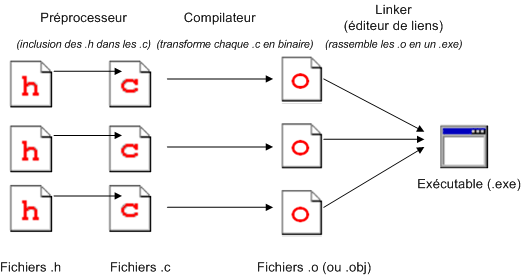
\includegraphics[width=13.5cm]{compilation.png}
	\caption{La compilation}
\end{figure}
\subsection{\'Etape 1 : Le préprocesseur}
Le pré processeur sont les instructions situés en dehors d'un programme, ceux-ci sont préfixé par un dièse (\#).
\begin{description}
	\item[Entrée] fichier.c
	\item[Sortie] fichier obtenu une fois les modifications effectués.
\end{description}~
\begin{lstlisting}[language=C, caption=Exemple d'instructions pré-processeurs]
#include // remplace par le continu du fichier inclus
#define Arg1 Arg2 // remplace syntaxique de Arg1 par Arg2
\end{lstlisting}
\subsection{Etape 2 : La compilation}
\begin{description}
	\item[Entrée] fichier.c, fichier.h
	\item[Sortie] fichier.o 
\end{description}
\begin{lstlisting}[language=bash]
gcc -c fic1.c fic2.c fic3.c # Créé les fichiers .c
gcc *.o nomExe #Créer l'executable.
\end{lstlisting}
\remarque{La compilation sera étudiée en détails lors des cours de L3 et M1}
\subsection{\'Etape 3 : L'édition de liens}
Rassemble tous les fichiers binaires .o en un seul executable.
	\chapter{Méthodologie de la programmation impérative}
		\section{Programmation ``en petit''}
		\begin{description}
			\item[Données] celle-ci son simple, comme un tableau à N éléments.
			\item[Problème] Petit.
			\item[Résolution] Développement d'un algorithme afin de traiter ces données.
		\end{description}
		Cf. cours du S3.

		\section{Programmation en large}
		\begin{description}
			\item[Données] celle-ci son complexes, modélisation des données avec des types abstrait.
			\item[Résolution] Développer de nombreux algorithmes afin de traiter le type abstrait. 
		\end{description}
		Cf. cours du S4.
		\section{Développement d'un algorithme}
		C'est un processus à 4 étapes:
		\begin{enumerate}
			\item \textbf{Comprendre} le problème : identifier le ``quoi''.
			\item \textbf{Spécification} du problème : formaliser le ``quoi''
			\item \textbf{Définir} un modèle de solution : identifier le ``comment''
			\item \textbf{Développer} et trouver l'algorithme : formaliser le ``comment''.
		\end{enumerate}

		\section{\'Etape 1 : comprendre le problème}
			Analyser du texte afin d'identifier les propriétés suivantes.
			\begin{itemize}
				\item Identifier les domaines du problèmes
			Le domaine pose les fondements scientifiques à utiliser par le programme. 
				\exemple{Arithmétique : se fonder sur la théorie du calcul\\ 
						Topologique: se fonder sur les bases mathématiques de topologie}
						\newpage

						Il faut se poser la question \textit{``est-ce calculable ?''} : est-ce que le problème peut être résolu par un ordinateur.
			\exemple{
				\begin{enumerate}
					\item Corriger toutes les fautes d'orthographe dans un texte: Non calculable car il y a un manque d'informations sur la taille et la nature des
			données.  
					\item Calculer la factorielle d'un entier $N \geq 0$ : calculable puisque la taille des données est fixée.
				\end{enumerate}
				}

			\item \textit{évaluer les contraintes ``Physiques''} liées au problème. 
				\begin{itemize}
					\item Les contraintes liées à l'architecture et au fonctionnement de l'ordinateur
					\item Les restrictions du problème.
				\end{itemize}

			\item Prendre des exemples et les traiter ``manuellement''
			\end{itemize}	

			En sortie de cette étape, nous avons une description informelle des données et de leur traitements.

		\section{\'Etape 2 : Spécification du programme : spécification formelle}
		Utilisation du langage logique des précédents pour écrire le programme, la spécification est composée de 3 informations appelée le triplet de \bsc{Hoare}.
			\begin{enumerate}
				\item Prédicat d'entrée : Exprime les propriétés logiques des données en entrée. 
				\item nomDuProgramme (données en entrée E, données en sortie) 
				\item Prédicat de sortie exprime les propriétés logiques des résultats.
			\end{enumerate}
			\exemple{
			Celui du facteur de $N \geq 0$
				\begin{itemize}
					\item $ N > 0 \wedge [(N \in N)] \wedge (N < 30)$
					\item \texttt{fact(N, f);}
					\item $f = N!$
				\end{itemize}
			}
			\section{\'Etape 3: Donner un modèle de solution}
			Exprimer les différentes étapes de transformation des données en entrée vers les données en sortie. 
			\begin{itemize}
				\item En langage naturel
				\item Sous forme fonctionnelle
			\end{itemize}
		\section{\'Etape 4 : Programmer et unifier le programme}	
		\begin{itemize}
			\item \'Ecriture en C du programme traduction du modèle vers le C.
				\subsubsection{Vérification du programme}
				\begin{itemize}
					\item Test d'exécution : Tableau de situation, vérification non exhaustive.
					\item Preuve formelle par calcul de ``Plus faible Pré condition'' (Pfp)
				\end{itemize}
				\paragraph{Le tableau de situation}
				\begin{description}
					\item[Données en entrée] Programme ``instrumenté'' : code source + point d'arrêt: 
						localisation dans l'espace du programme d'une opération de photographie de l'état de l'ordinateur.
					\item[Opération de transformation] Dénuder le programme et prendre les photos. 
					\item[Donnée en sortie] Liste de ``photos'' qui déçoit l'exécution de la même mémoire au cours de l'exécution.
				\end{description}
		\end{itemize}

	\chapter{Spécification d'un programme}
	\remarque{Durant ce chapitre, nous parlerons de programme, cependant cela est valable également pour les sous-programme}
	Un programme est spécifié par un triplet : 
	\begin{itemize}
		\item Prédicat d'entrée P(E) ou précondition
		\item action (E, S)
		\item Prédicat de sortie P(S) ou postcondition
	\end{itemize}

		Les prédicats sont écrits en utilisant le formalisme de la logique des prédicats et de sopérations booléeenes.
		\section{Mots clés à utiliser dans les prédicats}
		Les mots clés pouvant être utilisés: 
		\begin{itemize}
			\item Les quantificateurs logiques : $\forall$(quelque soit), $\exists$(il existe), $\nu$(nombre de)
			\item Les connecteurs logiques : $\wedge$(et), $\vee$(ou), $\rightarrow$(implique), $\leftrightarrow$(equivalence), $\lnot$(not)
		\end{itemize}
		\section{\'Ecriture de la spécification}
		C'es une traduction de l'énoncé et de l'analyse faite dans l'étape 1 de la méthodologie : c'est un \textbf{triplet} logique.
		La démarche pour écrire la spécification est la suivante.
			\begin{itemize}
				\item Identifier les propriétés des données d'entrée et les exprimer sous forme logique
				\item Identifier les propriétés sur les données en sortie et les exprimer sous forme logique. 
			\end{itemize}
		\exemple{
			\'Ecrire un programme qui trie un tableau T de N éléments.\\
			\begin{itemize}
				\item $N > 1$
				\item \texttt{trier (T, N, t);}
				\item $(\forall I : 0 \leq I < N-1 \longrightarrow T[I] \leq T[I+1]) \wedge$\\$
					(\forall I : 0 \leq I < N \longrightarrow $\\$(\nu J : 0 \leq J < N \wedge t[I] = t[J]) = (\nu J : o \leq J < N \wedge t[I] = T[J]))$ 
			\end{itemize}
		}
	
	\chapter{Vérification formelle de programmes}
	Vérifier que le programme est correct revient à démontrer l'implication suivante :\\ PE $\rightarrow$ pfp(\texttt{(action(D,r, PS);}

	Avec pfp étant la plus faible précondition\footnote{wp weakest precondition}.
	\begin{description}
		\item[pfp]	C'est un système de réécriture permetant de transformer une formule logique en une autre selon le programme qui doit s'éxécuter.
			C'est donc une réécriture syntaxique du prédicat de sortie en fonction des actions du programme.  \item[Tableau de situation] Système de réécriture des données en entrée (mémoireà vers les données en sortie (mémoire)) en fonction des actions du programme.  \end{description}
	\section{Système de réécriture Pfp}
		Ensemble de règles de réécriture permettant de transformer une formule logique en fonction des structures de base des langages de programmation.

		Les langages impératifs:
			\begin{itemize}
				\item affectation
				\item Séquence
				\item Sélection
				\item répétition
			\end{itemize}

		Règle de réécriture : \texttt{pfp(structure, formule) = formule}

	\section{Calcul de pfp d'une affectation}
	$$pfp("x=e", Q) = Q^e_n$$

	Avec la formule Q dans laquelle toutes les occurences de ``x'' sont remplacées par ``e'' (remplacement textuel)
	\exemple {
		Soit le programme suivant :
		\begin{itemize}
			\item $x > 0$
			\item $x = x-1$
			\item $x \geq 0$
		\end{itemize}
		On doit se poser la question \texttt{PE} $\rightarrow$ \texttt{pfp(programme, PS)} ?\\
		\begin{eqnarray*}
			(x > 0) &\rightarrow& \texttt{pfp}("x=x-1", x \geq 0)\\
			(x>0)&\rightarrow&(x-1 \geq 0)\\
			(x>0) &\rightarrow& (x > 0)
		\end{eqnarray*}
	}
	\section{Calcul du pfp d'une séquence}
	$$\texttt{pfp}("a1;a2;a3", Q) = \texttt{pfp}("a1;a2;", \texttt{pfp}("a3;", Q));$$
	\exemple{
	Soit les programme suivant, lesquels sont justes, lesquels sont faux ?
	\begin{itemize}
		\item \texttt{/* f = i! */}
		\item \texttt{i = i + 1;\\f = f*i}
		\item \texttt{/* f = i! */}
	\end{itemize}
\begin{eqnarray*}
	 f = i! &\rightarrow& \texttt{pfp}("i = i + 1 ; f = f \times i;", f = i!)\\
	 f = i! &\rightarrow& \texttt{pfp}("i = i +1", \texttt{pfp}("f = f \times i", f = i !)\footnote{\'Evaluation de la "règle" la plus profonde}\\
	 f = i! &\rightarrow& \texttt{pfp}("i = i+1", f \times i = i!)\\
	 f * i! &\rightarrow& f\times (i+1) = (i+1)!\\
	 &&i! \times(i+1) = (i+1)!\ \textmd{Par définition de}\ i!
\end{eqnarray*}

	\begin{itemize}
		\item \texttt{/* f = i! */}
		\item \texttt{f = f * (i + 1);\\i = i + 1;}
		\item \texttt{/* f = i! */}
	\end{itemize}
	\begin{eqnarray*}
		f = i! &\rightarrow& \texttt{pfp}("f = f\times (i+1); i = i +1;", f= i!)\\
		f=i!&\rightarrow&\texttt{pfp}("f=f\times(i+1);",\texttt{pfp}("i=i+1",f=i!)\\
		%f = i! &\rightarrow& \textt{pfp}("f = f \times (i + 1);" f = (i + 1)!)
	\end{eqnarray*}
	\begin{itemize}
		\item \texttt{/* (x = A) $\wedge$ (y = B) $\wedge$ (z = C)}
		\item \texttt{x = x + y +z;\\z = x - y - z;\\y = x - y -z;\\x = x - y - z;}
		\item \texttt{/* (x = B) $\wedge$ (y = C) $\wedge$ (z = A) */}
	\end{itemize}
	\begin{eqnarray*}
		PE &\rightarrow& \texttt{pfp}("x=x+y+z;z=x-y-z;y=x-y-z;x=x-y-z;", (x=B)\wedge(y=C)\wedge(z=A)\\
		PE &\rightarrow& \texttt{pfp}("x=x+y+z, z-x-y-z;y=x-y-z;", \texttt{pfp}("x=x-y-z;(x=B)\wedge(y=C)\wedge(z=A)\\
		PE &\rightarrow& \texttt{pfp}("x=x+y+z, z-x-y-z;y=x-y-z;", x-y-z=B)\wedge y=C \wedge z = A\\
		PE &\rightarrow& \texttt{pfp}("x=x+y+z,z=x-y-z", (y=B)\wedge (x-y-z=C)\wedge z = A\\
		PE &\rightarrow& \texttt{pfp}("x=x+y+z", (y=B)\wedge (z=C) \wedge (x-y-z=A)\\
		PE &\rightarrow& (y=B) \wedge (z=C)\wedge(x=A) \textmd{Vrai parceque }p\rightarrow p = vrai
	\end{eqnarray*}
	
}
\appendix



	\chapter{Glossaire}
	\paragraph{Compilation} Un compilateur est un programme informatique qui transforme un code source écrit dans un langage de programmation (le langage source) en un autre langage informatique (le langage cible).
	\paragraph{Interprétation}
	Analyse, traduit et exécute un programme écrit dans un langage informatique. De tels langages sont dits langages interprétés.

	L'interpréteur est capable de lire le code source d'un langage sous forme de script, habituellement un fichier texte, et d'en exécuter les instructions après une analyse syntaxique du contenu. Généralement ces langages textuels sont appelés des langages de programmation. Cette interprétation conduit à une exécution d'action ou à un stockage de contenu ordonné par la syntaxe textuelle.
	\paragraph{Édition de liens} Lors d’un développement informatique, l'édition des liens est un processus qui permet de créer des fichiers exécutables ou des bibliothèques dynamiques ou statiques, à partir de fichiers objets.
	\chapter{Exercices}
\section{Initiation}
	\subsection{Exercice 1}
\'Ecrire un programme qui lit une série de 10 valeurs et affiche la position du minimum et du maximum de la série.
\subsubsection{\'Etape 1: Analyser le problème}
\begin{enumerate}
	\item Lire les valeurs
	\item calculer les min et max
	\item afficher le résultat
\end{enumerate}
\subsubsection{\'Etape 2: Spécifier les sous-problèmes}
Identifier les entrée, les sorties et leurs propriétés.
\paragraph{\texttt{LireLesValeurs}}
\begin{description}
	\item[Entrée] Nombre, les valeurs à lire
	\item[Sortie] Tableau contenant les valeurs lues
\end{description}
\paragraph{\texttt{CalculerMinEtMax}}
\begin{description}
	\item[Entrée] Le tableau des valeurs et le nombre de valeur 
	\item[Sortie] Position, min et max. 
\end{description}
\newpage
\subsubsection{\'Etape 3: Le code}
\lstinputlisting[language=C, caption=Exercice 1 -- Code du programme]{annexes/exo1.c}
\newpage
\section{Tableau de situation}	
\subsection{Exercice 2}
\subsection{Exercice 3}

\lstinputlisting[language=C, caption=Exercice 3]{annexes/exo3.c}
\begin{center}
\begin{tabular}{c  |  c  c  c  c  }
\textbf{Point d'arrêt }& \textbf{T} & \textbf{j} & \textbf{i} &\textbf{n}\\
\hline
1 & 0,0,0,0,0 & 3 & 5 & 1\\
\hline
2 & 0,0,0,1,0 & 4 & 3 & @\\
\hline
3 & 5,9,1,1,1&4&5&\\
\hline
\end{tabular}
\end{center}
\newpage
\section{Effets de bords}
\subsection{Exercice 4}
\lstinputlisting[language=C, caption=Exercice 4]{annexes/exo4.c}
\begin{center}
\begin{tabular}{c |  c  c  c  c  c  c  }
	\textbf{Point d'arrêt} & \textbf{y} & \textbf{x} & \textbf{t} & \textbf{i} & \textbf{z} & \textbf{f}\\
	\hline
	2 & 10 & / & / & 1 && \\
	\hline
	1 & 11 & 1 & 2 & 1 & / & 13\\
	\hline
	3 & 11 & / & / & 1 & 24 & /\\
	\hline
\end{tabular}
\end{center}
\newpage
\subsection{Exercice 5}
\lstinputlisting[language=C, caption=Exercice 5]{annexes/exo5.c}
\begin{center}
\begin{tabular}{c |  c  c  c  c  c  }
	\textbf{Point d'arrêt} & \textbf{i} & \textbf{j} & \textbf{x} & \textbf{y} & \textbf{z}\\
	\hline
	3 & 3 & 7 &/ &/&/\\
	\hline
	1 & &&@i&@i&@j\\
	\hline
	2 & 6 & 12 & @i & @i & @j\\
	\hline
	4 & 6 & 12 & / & / & /\\
	\hline
	5 & 3 & 7 & / & / & / \\
	\hline
	1 & 3&10 &@j&@j&@i\\
	\hline
	2 & 20 & 10 & @j&@j&@i\\
	\hline
\end{tabular}
\end{center}
\newpage
\subsection{Exercice 6}
\lstinputlisting[language=C, caption=Exercice 6]{annexes/exo6.c} 
\begin{tabular}{c |  c  c  c  c  c  c  }
	\textbf{Point d'arrêt} & \textbf{i} & \textbf{j} & \textbf{x} & \textbf{a} & \textbf{a} & \textbf{f}\\
	\hline
	2&10&40&/&/&/&/\\
	\hline
	1 & 20 & 40 & / & 10 & 40 & 50\\
	\hline
	3 & 20 & 40 & 50 & / & / & /\\
	\hline
\end{tabular}

\section{Spécification}
\subsection{Exercice 7}
	\'Ecrire la spécification d'un programme qui dans un tableacu T de N entiers calcul le nombre n de nombre positifs dans le tableau.

	\begin{itemize}
		\item $N > 0$
		\item \texttt{calculeNbPos(T,N,n)}
		\item $(o \leq n \leq N) \wedge (n = \nu I : o \leq I < N T[I] \geq 0) $
	\end{itemize}
\subsubsection{Exercice 8}
	Soit T un tableau croissant (non strict) de N entier et X un entier.\\
	Spécifier un programme qui calcule la position de la dernière occurrence de T inférieure ou égale à X avec $T[0] \leq X < T[N-1]$

	\begin{itemize}
	%	\item $T[0] \leq X < T[N-1]$, $T[I] \leq T[I+1]$, $N > 0$
		\item $(N > 1) \wedge (T[0] \leq X) \wedge (X < T[N-1]) \wedge (\forall I : 0 \leq I < N - 1 \rightarrow T[I] \leq T[I+1])$
		\item \texttt{searchPosition(T, N, X, p));} 
		\item $(0 < p < N - 1) \wedge (T[p] \leq X) \wedge (T[p+1] > X)$
	\end{itemize}
	\remarque{Dans la suite du cours, nous pourrons utiliser un raccourcie afin de savoir si un tableau est trié par ordre croissant : $(T,N,\leq)$

	Celle-ci pourra être utilisée dans la copie à condition qu'elle soit définie au préalable.}

\subsection{Exercice 8}
	Soit un tableau T non vide de N entiers.  \'Ecrire la spécifications du qui programme qui calculent :
	\begin{itemize}
		\item La première position de la valeur max de T
		\item La dernière position de la valeur max de T
	\end{itemize}
	\subsubsection{Calcule de la première position}
	\begin{itemize}
		\item $N > 0$ 
		\item \texttt{searchFirstPosition(T, N, f);} 
		\item $(\forall I :0 \leq I < f \rightarrow T[I] < T[f]) \wedge (\forall I (f \leq I < N) \rightarrow (T[I] \leq T[f]))$ 
	\end{itemize}
	\subsubsection{Calcule de la dernière position}
	\begin{itemize}
		\item $N > 0$ 
		\item \texttt{searchLastPosition(T, N, l);} 
		\item $(\forall I :0 \leq I < l \rightarrow T[I] \leq T[l]) \wedge 
			(\forall I (l < I < N) \rightarrow (T[I] < T[l]))$ 
	\end{itemize}

\subsection{Exercice 9}
	\'Ecrire la spécification d'un programme qui, dans un tableau T de N entiers tous différents cherche la position d'une valeur X si elle existe ou retourne N si elle n'existe pas.

	\begin{itemize}
		\item $(N\geq0) \wedge (\forall I : 0 \leq I < N \rightarrow (\forall (I, J) : 0 \leq I < N \wedge (0 \leq J < N) \rightarrow T[I] = T[J] \leftrightarrow (I = J)$\footnote{Cela peut aussi s'écrire $N\leq 0) \wedge (\forall I (O \leq I < N) \rightarrow \forall J : J \neq I \wedge 0 \leq J < N \rightarrow T[I] \neq T[J]$}
		\item \texttt{search(T, N, x)}
		\item $(0 \leq p < N \wedge T[p] = X) \vee (p=N) \leftrightarrow \forall I (o\leq I < N) \rightarrow T[I] \neq X))$ 
	\end{itemize}

	\subsection{Exercice 10}
	Spécifier un programme qui, dans un tableau T de N éléments trié par ordre croissant non strict retourne la longueur du plus grand plateau\footnote{Un plateau est quand il y a plusieurs fois le même caractère}.

\begin{itemize}
	\item $(T, N, \leq) \wedge N > 0$
	\item \texttt{longueurPlusGrandPlateau(T,N,l);}
	\item $(1 \leq l \leq N) \wedge (\exists I : 0 \leq I < N-l)\wedge (T[I] = T[I+l-1])$ 
\end{itemize}
	\subsection{Exercice 11}
		Spécifier un programme qui, dans un tableau de N entiers calcule le nombre de doublons : un doublon est une succession de 2 nombres identiques.

		\begin{itemize}
			\item $N > 0$
			\item \texttt{calculeDoublons(T, N, n);}
			\item $n = \nu I : 0 \leq I < N \wedge T[I] = T[I+1]$
		\end{itemize}
		\remarque{
			Dans le cas ou deux doublons ne sont pas forcément côte à côte, le prédicat de sortie deviendrait : 
			$$n = \sum^{N-1}_{I=0} \nu J : I < J < N \wedge T[J] = T[I]$$
		}

\section{Preuves de programmes}
\subsection{Séquence}\label{exoPfpSequence}
\begin{itemize}
	\item \texttt{/* f = i! */}
	\item \texttt{f = f * (i + 1);\\i = i + 1;}
	\item \texttt{/* f = i! */}
\end{itemize}
\begin{eqnarray*}
	f = i! &\rightarrow& \texttt{pfp}("f = f\times (i+1); i = i +1;", f= i!)\\
	f=i!&\rightarrow&\texttt{pfp}("f=f\times(i+1);",\texttt{pfp}("i=i+1",f=i!)\\
	%f = i! &\rightarrow& \textt{pfp}("f = f \times (i + 1);" f = (i + 1)!)
\end{eqnarray*}
\begin{itemize}
	\item \texttt{/* (x = A) $\wedge$ (y = B) $\wedge$ (z = C)}
	\item \texttt{x = x + y +z;\\z = x - y - z;\\y = x - y -z;\\x = x - y - z;}
	\item \texttt{/* (x = B) $\wedge$ (y = C) $\wedge$ (z = A) */}
\end{itemize}
\begin{eqnarray*}
	PE &\rightarrow& \texttt{pfp}("x=x+y+z;z=x-y-z;y=x-y-z;x=x-y-z;", (x=B)\wedge(y=C)\wedge(z=A)\\
	PE &\rightarrow& \texttt{pfp}("x=x+y+z, z-x-y-z;y=x-y-z;", \\&&\texttt{pfp}("x=x-y-z;(x=B)\wedge(y=C)\wedge(z=A)\\
	PE &\rightarrow& \texttt{pfp}("x=x+y+z, z-x-y-z;y=x-y-z;", x-y-z=B)\wedge y=C \wedge z = A\\
	PE &\rightarrow& \texttt{pfp}("x=x+y+z,z=x-y-z", (y=B)\wedge (x-y-z=C)\wedge z = A\\
	PE &\rightarrow& \texttt{pfp}("x=x+y+z", (y=B)\wedge (z=C) \wedge (x-y-z=A)\\
	PE &\rightarrow& (y=B) \wedge (z=C)\wedge(x=A) \textmd{Vrai parceque }p\rightarrow p = \textmd{vrai}
\end{eqnarray*}

\subsection{Sélection} \label{exoPfpSelect}
\subsubsection{Exercice 1}
\begin{lstlisting}[language=C]
/* x = A */
if(x < 0)
x = -x;

/* x = |A| */
\end{lstlisting}

\begin{eqnarray*}
/*x = A*/ &\rightarrow& \pfp ("if(x < 0)\{ x = -x \}", x = |A|)\\
/*x = A*/ &\rightarrow& (((x<0)\rightarrow \pfp ("x=-x;", x = |A| ) \wedge (x >= 0 \rightarrow x = |A|)))\\
/*x = A*/ &\rightarrow& (((x < 0) \rightarrow (-x = |A|)) \wedge (( x >= 0) \rightarrow (x = |A|)))\\
\end{eqnarray*}
$( A ( A < 0) \rightarrow (-A = |A|) ) \wedge (A >= 0 \rightarrow (A=|A|))$
Définition de la valeur absolue $|.|$.

\subsubsection{Exercice 2}
\begin{lstlisting}[language=C]
/* x = A $\wedge$ y = B */
if (A < B) {
x = A;
y = B;
} else {
x = B;
y = A;
}
/* x $\leq$ y */ 
\end{lstlisting}
\begin{eqnarray*}
PE &\rightarrow& \pfp ("\ifp (A < B) \{ x = A; y = B\}\elsep \{ x = B; y =A\}", x \leq y)\\
PE&\rightarrow&((A<B)\rightarrow\pfp("x=A;y=B",x\leq y))\wedge((A\geq B)\rightarrow\pfp("x=B;y=A",x\leq y))\\
PE &\rightarrow& ((( A < B) \rightarrow (A \leq B)) \wedge (A \geq B ) \rightarrow (B \leq A))
\end{eqnarray*}
Vrai par définition. A et toujours inférieur à B. $(A \geq B) \rightarrow (B \leq A)$ est une Tautologie. 
\subsubsection{Exercice 3}
$$\pfp ("\ifp (x \geq y )\{z=x;\}\elsep\{z=y\}",z=\texttt{max}(x,y))$$
\begin{eqnarray*}
x \geq y  &\rightarrow&	\pfp ("\ifp (x \geq y )\{z=x;\}\elsep\{z=y\}",z=\texttt{max}(x,y))\\
x \geq y &\rightarrow& \pfp ("z = x", z = \texttt{max}(x,y))\\
x < y &\rightarrow& \pfp ("z = y", z = \texttt{max}(x,y))\\
x \geq y &\rightarrow& x = \texttt{max}(x,y)\\
x < y &\rightarrow& y = \texttt{max}(x,y)
\end{eqnarray*}
C'est une tautologie par définition de \texttt{max}.

\subsubsection{Exercice 4}
$$\pfp ("\ifp (x > y) \{ if(x \%2 ==  0) \{ x = x - 2\}\} \elsep \{y=y-1;\}", y-2 < x);$$
\begin{eqnarray*}
(x > y) &\rightarrow& \pfp("if(x\%2 == 0) { x = x-2; } ", y-2 < x)) \wedge ( ( x \leq y) \rightarrow \pfp ("y = y-1;", y - 2 < x) )\\
(x > y) &\rightarrow& ( ( (x \%2 = =0) \rightarrow \pfp ("x = x-2", y-2 < x) \wedge \\
& &(x \% 2 != 0) \rightarrow(y-2 < x)) \wedge ( (x \leq y) \rightarrow (y-z < x))\\ 
(x > y) &\rightarrow& ( (x\%2 = = 0)\rightarrow ( (y-2) < (x - 2) ) \wedge ( ( x\%2 != 0) \rightarrow (y-2 < x))) \wedge (x \leq y \rightarrow y-z < x) \\
(x > y) &\rightarrow& (x \leq y \rightarrow y - z < x)
\end{eqnarray*}
\subsection{Boucles}\label{exoPfpBoucles}
\subsubsection{Exercice 1}
\begin{lstlisting}[language=C]
/* $N \geq 0$ */

/* P Tableau de polynôme
* N Degré du polynôme
* X Point ou je veux évoluer le polynôme
* r Résultat du polynôme
*/
calculPolynome(P,N,X,r);
/* $r = \sum^N_{k=0} A[I]X^k $ */
\end{lstlisting}
\begin{lstlisting}[language=C]
/* $N \geq 0$ */

/*	INV = $(o \leq i \leq N) \wedge (r = \sum^i_{k=0} A[k]x^k) \wedge (y = x^i)$*/
while(c) {
/* c \wedge INV */
corps;
/* INV */
}
/* $\neg c \wedge INV$ */
/* $p = \sum^N_{k=0} A[k] x^k$ */
\end{lstlisting}
\paragraph{INVARIANT}
$$(o \leq i \leq N) \wedge (r = \sum^i_{k=0} A[k]x^k) \wedge (y = x^i)$$
\paragraph{Intitialisation}
\begin{enumerate} 
	\item INIT 0 \begin{lstlisting}[language=C,numbers=none]
i = 0; 
p = 0; 
y = 1;
\end{lstlisting}~
\begin{eqnarray*}
PE &\rightarrow& \pfp (\texttt{init}\ 0, \texttt{INV})\\
N \geq 0 &\rightarrow& \pfp ("i=0;p=0", p=\sum^i_k=0 A[k]x^k \wedge 1 = x^i);\\
N \geq 0 &\rightarrow& \pfp ("i=0", 0 = \sum^i_{k=0} A[k]x^k \wedge 1 = x^i\\
N \geq 0 &\rightarrow& 0 = \sum^0_{k=0} A[k]x^k \wedge 1 = x^0\\
(N \geq 0 &\rightarrow& 0 = A[0] \wedge 1 = 1) \Rightarrow \textrm{Faux et Vrai, donc le programme est Faux} \end{eqnarray*}
	\item INIT 1 \begin{lstlisting}[language=C,numbers=none]
i = 0; 
p = A[0]; 
y = 1;
\end{lstlisting}
\begin{eqnarray*}
PE &\rightarrow& \pfp (\texttt{init}\ 1, \texttt{INV})\\
N \geq 0 &\rightarrow& \pfp ("i=0;p=A[0]", p=\sum^i_k=0 A[k]x^k \wedge 1 = x^i);\\
N \geq 0 &\rightarrow& \pfp ("i=0", A[0] = \sum^i_{k=0} A[k]x^k \wedge 1 = x^i\\
N \geq 0 &\rightarrow& A[0] = \sum^0_{k=0} A[k]x^k \wedge 1 = x^0\\
(N \geq 0 &\rightarrow& A[0] = A[0] \wedge 1 = 1) \Rightarrow \textrm{Vrai et Vrai, donc le programme est correct}
\end{eqnarray*}
\end{enumerate}
L'initialisation nécessaire est donc init 1.
\paragraph{Boucles} 
\begin{enumerate} 
	\item \begin{lstlisting}[language=C,numbers=none]
while(i < N) { 
++i; 
p = p + A[i-1] * y; 
y = y * X; 
}
	\end{lstlisting}~
	\'Etape numéro \ref{etape3boucle} (Cf section \ref{pfpBoucle} page \pageref{etape3boucle})
	\begin{eqnarray*}
		\neg C \wedge INV &\rightarrow& PS\\
		(i > N) \wedge (p = \sum^i_{k=0} A[k] x^k) \wedge(y=x^i) &\rightarrow& p = \sum^N_{k=0}A[k]x^k\\
		(i > N) \wedge (p = \sum^i_{k=0} A[k] x^k) \wedge(y=x^i) &\rightarrow& p = \sum^N_{k=0}A[k]x^k\wedge (i=N)\\
		(i > N) &\rightarrow& (i = N) \Rightarrow \textrm{C'est donc faux.}\\
	\end{eqnarray*}
	\remarque{Nous sommes partis de la conclusion et avons essayé de faire apparaitre notre hypothèse en partie droite.}
	\item \begin{lstlisting}[language=C,numbers=none]
while( i != N) { 
++i; 
p = p + a[i-1] * y; 
y = y * X 
} 
\end{lstlisting}~
	\'Etape numéro \ref{etape3boucle} (Cf section \ref{pfpBoucle} page \pageref{etape3boucle})
	\begin{eqnarray*}
		\neg C \wedge INV &\rightarrow& PS\\
		(i \neq N) \wedge (p = \sum^i_{k=0} A[k] x^k) \wedge(y=x^i) &\rightarrow& p = \sum^N_{k=0}A[k]x^k\\
		(i \neq N) \wedge (p = \sum^i_{k=0} A[k] x^k) \wedge(y=x^i) &\rightarrow& p = \sum^N_{k=0}A[k]x^k\wedge (i=N)\\
		(i \neq N) &\rightarrow& (i = N) \Rightarrow \textrm{C'est donc vrai}. 
	\end{eqnarray*}
	\'Etape numéro \ref{etape2boucle} (Cf section \ref{pfpBoucle} page \pageref{etape3boucle})
	\begin{eqnarray*}
		C \wedge INV &\rightarrow& \pfp(corps, INV)\\
		C \wedge INV &\rightarrow& \pfp ("i++;p=p+A[i-1]*y;", (p=\sum^i_{k=0}A[k]x^k)\\&&\wedge(y*x=x^i)\wedge(0\leq i\leq n )\\
		C \wedge INV &\rightarrow& \pfp ("i++;", (p+A[i-1]*y = \sum^i_{k=0}A[k]x^k)\\&&\wedge(y*x=x^i)\wedge(0\leq i\leq n )\\
		(i \neq N) \wedge (0\leq i \leq N) \wedge\\ (p = \sum^i_{k=0} A[k] x^k) \wedge (y=X^i) &\rightarrow& (p+A[i] * i = \sum^{i+1}_{k=0}A[k]x^k) \wedge (y \times x = x^{i+1}) \wedge (0 \leq i+1 \leq N)\\
		(i \neq N) \wedge (0\leq i \leq N) \wedge \\(p = \sum^i_{k=0} A[k] x^k) \wedge (y=X^i) &\rightarrow& A[i] \times x^i = p+A[i+1]x^{i+1} \wedge x^i \times = x^{i+1} \wedge Tautologie \\
		(i \neq N) \wedge (0\leq i \leq N) \wedge \\(p = \sum^i_{k=0} A[k] x^k) \wedge (y=X^i) &\rightarrow& Faux \wedge Tautologie \wedge Tautologie\Rightarrow \textrm{Le programme est donc faux} \\
	\end{eqnarray*}
\item \begin{lstlisting}[language=C,numbers=none]
while(i == N) { 
++i;	
p = p +(A[i] * y * X); 
y = y * X; 
}
\end{lstlisting}
Ce programme effectue la correction de l'erreur détectée plus haut. Il est correct.
\end{enumerate}

\subsubsection{Exercice 2 : Suite de Fibonacci}
\remarque{
Le rang $n$ de la suite de Fibonacci est défini comme suit: \\
$F_n = 1$ si $n=0$ ou $n=1$\\
$F_n = F_n-2 + F_n-1$ si i$n > 1$}

\begin{lstlisting}[language=C,numbers=none]
/* $N \geq 0$ */
i = 0; 
a = 1; 
b = 1;
/* $INV = (F_i = a) \wedge (F_n-1 = b) \wedge (o \leq i \leq N)$ */
while(c) {
/* $c \neg INV$ */
i++;
b += a;
a = b - a;
/* $INV$ */
}
/* $\neg c \wedge INV$ */
/* $F_n = \{\cdots\}$ */
\end{lstlisting}

\remarque{Il est conseillé de commencer par l'étape la plus facile, en effet, une étape et nous n'avons pas à effectuer les autres}
\paragraph{Etape 1}
\begin{eqnarray*}
PE &\rightarrow& \pfp("init", INV)\\
N \geq 0 &\rightarrow& (F_{i+1} = 1) \wedge (F_i = 1) \wedge (i=0)\\
N \geq 0 &\rightarrow& (F_1 = 1) \wedge (F_0 = 1)\Rightarrow \textrm{Tautologie par définition}
\end{eqnarray*}
\paragraph{Etape 3}
\begin{eqnarray*}
(i = N) \wedge (F_i = a) \wedge (F_{i+1} = b) \wedge (0 \leq i \leq N) &\rightarrow& F_N = a\\
(F_n = a) \wedge (F_{N+1}) \wedge (0 \leq N) &\rightarrow& F_N = a \Rightarrow \textrm{Tautologie}
\end{eqnarray*}

\paragraph{Etape 2}
\begin{eqnarray*}
(i \neq N) \wedge (F_i = a) \wedge (F_{i+1} = b) \wedge (0 \leq i \leq N) &\rightarrow& \pfp("\cdots", F_i=b-a \wedge F_{i+1} = b \wedge \cdots)\\
&\rightarrow& \pfp ("\cdots", F_i = b+a - a \wedge F_{i+1} = b+a\\
&\rightarrow& F_i+1 = b \wedge F_{i+2} = b + a \wedge i+1 \leq N\\
&\rightarrow& T \wedge T \textrm{par définition} \wedge T 
\end{eqnarray*}

\paragraph{Etape 4}
Tester une existance de $f > 0$ avant l'execution du corps : $c \wedge INV \rightarrow f > 0$.
\begin{eqnarray*}
(i \neq  N) \wedge (F_i = a) \wedge (F_n-1 = b) \wedge (o \leq i \leq N) &\rightarrow& f > 0\\
 f = N-i \Rightarrow N \geq 0\textrm{ donc Vrai.}
\end{eqnarray*}

\paragraph{\'Etape 5}
\begin{eqnarray*}
f = F \wedge c \wedge INV &\rightarrow& \pfp("corps", f < F)\\
N-i = F \wedge c \wedge INV &\rightarrow& \pfp("corps", N-i < F)\\
N - i = F \wedge c \wedge INV &\rightarrow& N - (i+1) < F\\
&\rightarrow& N -i-1 < F \\
&\rightarrow& F-1 < F \Rightarrow \textrm{Tautologie}
\end{eqnarray*}

\subsubsection{Exercice 3 : plus grand plateau}
\begin{lstlisting}[language=C]
	/* $(N \geq 1) \wedge (B(N), \geq )$ */
	j = 1;
	p = 1;
	/* $INV = (1 \leq p \leq j \leq N) \wedge (\exists k : 0 \leq k \leq j - p) \wedge (B[k] = B[k+p-1]))$
	$\wedge (\forall k (0 \leq k \leq j -p - 1) \rightarrow (B[k] \neq B[k+p]))$ */
	while (j != N) {
		/* $INV \wedge c$ */
		if(B(j-p] == B[j]) 
			p++;

		j++;
		/* INV */
	}
	/* $\neg c \wedge INV$ */
	/* $R = (1 \leq p \leq N) \wedge (\exists k : 0 \leq k \leq N - p) \wedge $
	$(B[k] = B[k+p-1])) \wedge (\forall k (0 \leq k \leq N -p - 1) \rightarrow (B[k] \neq B[k+p]))$ */
\end{lstlisting}
\remarque{$(B(N), \geq)$ signifique le tableau est ordonné dans l'ordre croissant non strict}

Soit PE le prédicat d'entrée.


\begin{eqnarray*}
	x \geq 1 &\rightarrow& \pfp (j=1,p=1, Inv)\\
	x \geq 1 &\rightarrow& (0 \leq 1 \leq 1 \leq N)\wedge \exists k(0 \leq k \leq 0 (B[k]=B[k])) \wedge \forall k(0 \leq k \leq -1 \rightarrow B[k] \neq B[k+1]\\
	&& \Rightarrow \textrm{ Toujours vrai }
\end{eqnarray*}

\begin{eqnarray*}
	C \wedge INV &\rightarrow& \pfp (\ifp (B[j-p] == B[k]) p++;j++,INV)\\
	C \wedge INV &\rightarrow& \pfp (\ifp(B[j-p] == B[j]) p++, \pfp(j++, INV))\\
	C \wedge INV &\rightarrow& \pfp(\cdots
	, 1 \leq p \leq j+1 \leq N \wedge \exists k (0 \leq k\leq j + 1 - p)\\&&
			\wedge B[k] = B[k+p-1] \wedge \exists \forall k(0 \leq k < j+1-p-1 \rightarrow B[k] \neq B[k+p] )) = A\\
C \wedge INV &\rightarrow& B[j-p] == B[j] \rightarrow \pfp (p++, A) \wedge B[j-p]  \neq B[j] \rightarrow A\\
C \wedge INV &\rightarrow& (B[j-p] \neq B[j] \rightarrow (0 \leq p \leq j+1 \leq N) \wedge \exists k 0 \leq k \leq j+1-p \wedge B[k] = B[k+p-1] \\&&
\wedge \forall k 0 \neq k \leq j-p \rightarrow B[k] \neq B[k-p]\\
&\rightarrow& T \wedge \exists k 0 \leq k< j-p \wedge B[k] = B[k+1-p] \wedge B[j+1-p] = B[j+1-p+1-p] \wedge \cdots\\
\end{eqnarray*}
\subsubsection{Exercice 4 : Définition variante}
\begin{eqnarray*}
	C \wedge INV &\rightarrow& f > 0\\
	J \neq N \wedge INV &\rightarrow& (f = N-j) >0 \Rightarrow \textrm{ Vrai }
\end{eqnarray*}

\begin{eqnarray*}
	N-j  =F \wedge C \wedge INV &\rightarrow& \pfp(corps, N-j < F)\\
	N-j  =F \wedge C \wedge INV &\rightarrow& \pfp(\ifp(\cdots))\cdots,\pfp(j++,N-j<F)\\
	N-j  =F \wedge C \wedge INV &\rightarrow& B|j-p] = B[j] \rightarrow N - j -1 < F \wedge B[j-p] \neq B[j] \rightarrow N-j-1 < F\\
	N-j = F \wedge C \wedge INV \rightarrow N-j-1 < F \wedge F-1 < F
\end{eqnarray*}

\subsubsection{Exercice 5}

\begin{lstlisting}[language=C]
	/* $A \leq 0 \wedge B \geq 0 */
	x = A;
	y = B;
	z = 1;

	/* (z = x^y = A^B) \wedge y \geq 0$ */
	while(y != 0) {
		/* $z *x^y = A^B \wedge y \geq 0$ */
		while(y \% 2 == 0) {
			y = y / 2 ;
			x = x*x;
		}
		/* $z = x^y = A^B \wedge y > 0 \wedge y \%2 \neq 0 $*/
		y--;
		z = z * x;
		/* z = x^y = A^B \wedge y \geq 0 */
	}
	PS : /* z = A^b */

\end{lstlisting}
\section{\'Ecriture d'un programme à partir de sa preuve}
\subsection{Exercice 1 : Dichotomie}
\begin{lstlisting}[language=C]
/* N > 0 */
a = 1;
b = N;
while(b != a + 1) {
	m = (a+b)/2;
	if(0 <= N-m*m) {
		a = m;
	} else {
		b = m;
	}
}
/*
 * Réécriture : $a^2 \leq N \wedge N \leq b^2 \wedge (b=a+1)$
 * $a^2 \leq N \wedge N \leq (A+1)^2$  
 */
\end{lstlisting}
Variante : $b-a$ : taille de l'intervalle. Fonction décroissante.
\subsection{Exercice 2}

\begin{lstlisting}[language=C]
/* N $\leq$ 2 $\wedge$ B(0..N-1, $\leq$) $\wedge$ B[0] $\leq$ X $\wedge$ B[N-1] > X */
cherchep(B,N,X,p);
p = 0; 
/* 0 $\leq$ p $\leq$ i-2 $\wedge$ B(p) $\leq$ x $\wedge$ B[p+1] > x */ 
while (B[p+1] <= X) {
	++p;
}
/* 
 * 0 $\leq$ p $\leq$ N-2 $\wedge$ B[p] $\leq$ x < B[p+1] 
 */
\end{lstlisting}
Variante : $N - i$

	\lstlistoflistings{}

\end{document}






